% -*- TeX:de -*-
\NeedsTeXFormat{LaTeX2e}
\documentclass[12pt,a4paper,titlepage]{article}

%\usepackage[german]{babel} % german text
\usepackage[DIV12]{typearea} % size of printable area
\usepackage[T1]{fontenc} % font encoding
\usepackage[utf8]{inputenc} % probably on Linux

\usepackage{graphicx} % to include images
\graphicspath{ {img/} } % set default image directory
\usepackage{subfigure} % for creating subfigures
\usepackage{amsmath} % a bunch of symbols
\usepackage{amssymb} % even more symbols
\usepackage{booktabs} % pretty tables
\usepackage{csquotes}

% a floating environment for circuits
\usepackage{float}
\usepackage{caption}

\newfloat{circuit}{tbph}{circuits}
\floatname{circuit}{Schaltplan}

% a floating environment for diagrams
\newfloat{diagram}{tbph}{diagrams}
\floatname{diagram}{Diagramm}

\renewcommand{\familydefault}{\sfdefault} % activate to use sans-serif font as default

\sloppy % friendly typesetting

\usepackage{eurosym}
\usepackage{makeidx}
\usepackage{amsfonts}
\usepackage{mparhack}
\usepackage{array}
\usepackage{tabularx}
\usepackage{minitoc}
\usepackage[colorlinks=true]{hyperref}
\usepackage{epstopdf}
\usepackage{setspace}
\usepackage{csquotes}
\usepackage{circuitikz}

% hyperref settings
\hypersetup{
    colorlinks=false,       % false: boxed links; true: colored links
    linkcolor=black,          % color of internal links (change box color with linkbordercolor)
    citecolor=black,        % color of links to bibliography
    filecolor=black,      % color of file links
    urlcolor=black           % color of external links
}

\begin{document}

\begin{titlepage}

\begin{figure*}[h!]
  
\includegraphics[width=8cm]{TULogo_CMYK}
\end{figure*}

\begin{center}
\vspace*{1.3cm}
{\Huge Elektrotechnische Grundlagen der Informatik\\(LU 182.692)\\}
\vspace{1.7cm}
{\LARGE Protokoll der 3. Labor\"ubung: \enquote{OPV}\\}
{\large \enquote{Transiente Vorg\"ange und Frequenzverhalten}\\}
{\LARGE b) Messungen\\}
\vspace{1.5cm}

% fill in group number and date of lab here
% CHANGE ME!
{\Large Gruppennr.: 22 \hspace{1cm} Datum der Labor\"ubung: 01.06.2017}

% fill in IDs and names here
% CHANGE ME!
\begin{table}[h!]
\centering
\begin{tabular}{|p{3.5cm}|p{3.5cm}|p{6.5cm}|}
\hline \textbf{Matr. Nr.} & \textbf{Kennzahl} & \textbf{Name} \\
\hline
1614835 & 033 535 & Jan Nausner \\
\hline
1633068 & 033 535 & David Pernerstorfer \\
\hline
\end{tabular}
\end{table}

\end{center}
\vspace{1.0cm}

\begin{table}[h!]
\begin{tabular}{|l|l|}
\hline \textbf{Kontrolle} & \checkmark \\
\hline Nichtinvertierender OPV & \\
\hline OPV und Grenzfrequenz & \\
\hline Invertierender OPV & \\
\hline Integrierer & \\
\hline Schmitt-Trigger & \\
\hline
\end{tabular}
\end{table}

\end{titlepage}
% start of actual lab protocol
% CHANGE ME!

\setcounter{page}{2}

\newpage
\setcounter{tocdepth}{1}
\tableofcontents

\newpage

\section*{Materialien}
\begin{itemize}
	\item Oszilloskop: Agilent InfiniiVision MSO-X 3054A
	\item Frequenzgenerator: Agilent 33220A
  \item Netzteil Agilent U8031A
  \item Multimeter: Amprobe 37XR-A
\end{itemize}

\section{Nichtinvertierender OPV}

\subsection*{Aufgabenstellung}
Durch Messung der Ströme und Spannungen an einem nichtinvertierenden OPV soll dessen Verhalten nachvollzogen werden.

\subsection*{Schaltplan}
\begin{figure}[H]
  \centering
  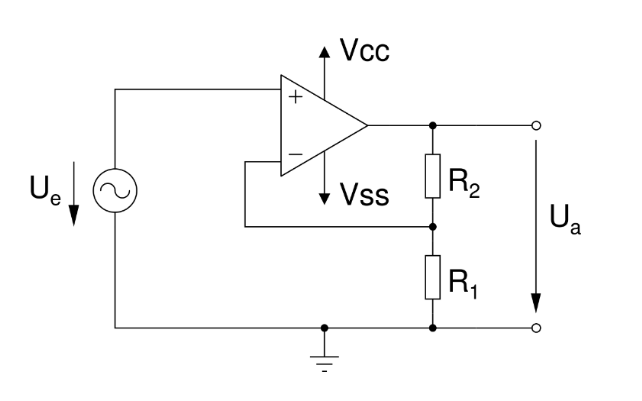
\includegraphics[width=100mm]{ni_opv_schaltung.png}
  \caption{Nichtinvertierender OPV}
\end{figure}

\subsection*{Durchf\"uhrung}
Die Schaltung wurde gemäß Schaltplan mit dem OPV-IC LM741 aufgebaut. Die Widerstände wurden mit $R_1 = 1k\Omega$ und $R_2 = 47k\Omega$ gewählt um gemäß der Übertragungsfunktion der Schaltung

\begin{figure}[H]
  \centering
  $U_a = U_e(1+\frac{R_2}{R_1}) = U_e(1+\frac{47k\Omega}{1k\Omega}) = 48*U_e$
\end{figure}

\noindent eine 48-fache Verstärkung der Eingangsspannung zu erreichen. Der OPV wurde mit $\pm 15V$ Versorgungsspannung betrieben. Um Ströme und Spannungen in der Schaltung zu messen, wurde ein Eingangsspannung von $0,1V$ angelegt und die Werte in der Folge mit dem Multimeter erhoben. Dieselben Messungen wurden mit einer Eingangsspannung von $0,3V$ wiederholt. Um das Verhalten des nichtinvertierenden OPV im Zeitbereich zu untersuchen, wurde eine Rechteckspannung mit $0,1V_{pp}$ Amplitude und jeweils mit $100Hz$ und $10kHz$ Frequenz angelegt. Hierbei wurden Messungen mit dem Oszilloskop durchgeführt.

\subsection*{Ergebnisse \& Diskussion}

% \begin{table}[H]
%   \centering
%   \begin{tabular}{c||c|c||c|}
%     & $U_e = 0,1V$ & Abweichung & $U_e = 0,3V$\\
%     \hline
%     $U_a$ & $5,43V$ & $+13,1\%$ & $14,21V$ \\
%     \hline
%     $U_{R2}$ & $4,43V$ & $-5,7\%$ & $13,91V$ \\
%     \hline
%     $U_{R1}$ & $100mV$ & $\pm 0\%$ & $293mV$\\
%     \hline
%     $U_d$ & $-0,8mV$ & $-1160\%$ & $5mV$ \\
%     \hline
%     $I_{R2}$ & $105mA$ & $+1050\%$ & $-279uA$ \\
%     \hline
%     $I_{R1}$ & $102mA$ & $+1020\%$ & $-280uA$ \\
%     \hline
%     $I_{+}$ & $0,15uA$ & $+12,5\%$ & $0,07uA$ \\
%     \hline
%     $I_{-}$ & $-0,04uA$ & - & $-0,11uA$ \\
%   \end{tabular}
%   \caption{Messergebnisse bei Gleichspannung mit Abweichungen zur Simulation}
% \end{table}

\begin{table}[H]
  \centering
  \begin{tabular}{c|c|c}
    & $U_e = 0,1V$ & $U_e = 0,3V$\\
    \hline
    $U_a$ & $5,43V$ & $14,21V$ \\
    \hline
    $U_{R2}$ & $4,43V$ & $13,91V$ \\
    \hline
    $U_{R1}$ & $100mV$ & $293mV$\\
    \hline
    $U_d$ & $-0,8mV$ & $5mV$ \\
    \hline
    $I_{R2}$ & $105uA$ & $-279uA$ \\
    \hline
    $I_{R1}$ & $102uA$ & $-280uA$ \\
    \hline
    $I_{+}$ & $0,15uA$ & $0,07uA$ \\
    \hline
    $I_{-}$ & $-0,04uA$ & $-0,11uA$ \\
  \end{tabular}
  \caption{Messergebnisse bei Gleichspannung}
\end{table}

\noindent Die Verstärkung eines Idealen OPV ist unendlich groß, sie wird jedoch durch die Beschaltung herabgesetzt. Die berechnete Verstärkung der Schaltung beträgt $48$, bei $U_e = 0,1V$ beträgt die gemessene Verstärkung $54,3$ und bei $U_e = 0,3V$ $47$. Da der Ideale OPV einen unendlich großen Eingangswiderstand hat, kann man auch hier erkennen, dass an den Eingängen nur ein sehr kleiner Strom fließt. Die Differenzspannung, welche beim idealen OPV $0V$ beträgt ist mit $-0,8mV$ bzw. $5mV$ bei der realen Beschaltung auch sehr klein. Man erkennt, dass an $R_1$ die Eingangspannnung abfällt. %Anhand der Messungen lässt sich vermuten, dass der LM741-OPV bei $0,3V$ Eingangspannung näher an das Verhalten eines idealen OPV herakommt als bei $0,1V$ Eingangsspannung.

\begin{figure}[H]
  \centering
  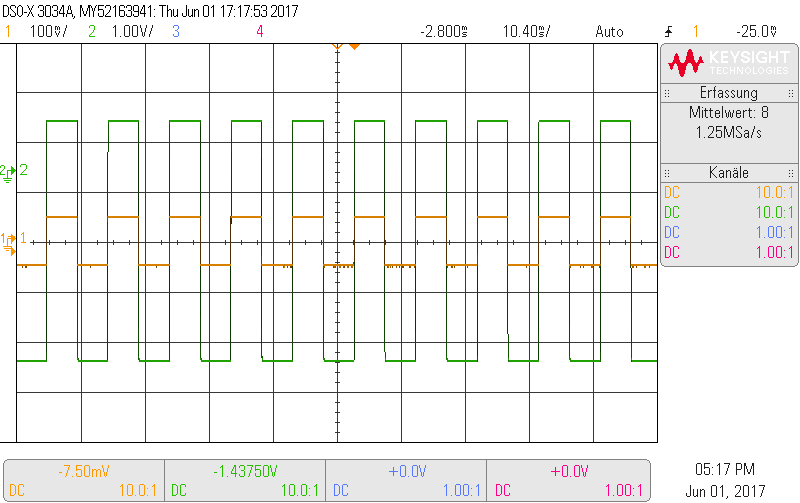
\includegraphics[width=150mm]{scope_0.png}
  \caption{Rechtecksignal mit $100Hz$ (gelb $\hdots\;U_e$, grün $\hdots\;U_a$)}
\end{figure}

\begin{table}[H]
  \centering
  \begin{tabular}{c|c|c}
     & $pp$ & $RMS$ \\
     \hline
    $U_{e}$ & $100mV$ & $49,7mV$ \\
    \hline
    $U_{a}$ & $4,8V$ & $2,4V$
  \end{tabular}
  \caption{Messungen mit Oszilloskop}
\end{table}

\noindent Das Rechteckssignal am Eingang wird am Ausgang 48-fach verstärkt, wie man anhand der Spitze-Spitze-Spannungen erkennen kann. Das Signal am Ausgang entspricht ebenfalls einem Rechteck. Ein- und Ausgangsspannung sind phasengleich.

\begin{figure}[H]
  \centering
  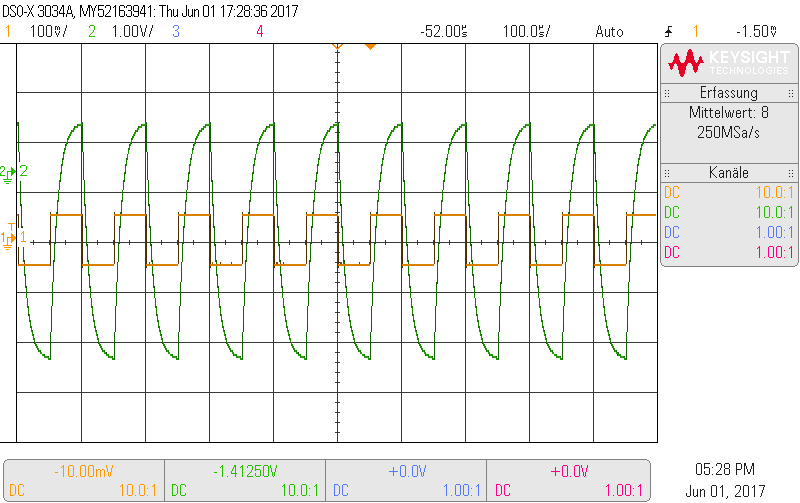
\includegraphics[width=150mm]{scope_3.png}
  \caption{Rechtecksignal mit $10kHz$ (gelb $\hdots\;U_e$, grün $\hdots\;U_a$)}
\end{figure}

\begin{table}[H]
  \centering
  \begin{tabular}{c|c|c}
     & $pp$ & $RMS$ \\
     \hline
    $U_{e}$ & $100mV$ & $49,7mV$ \\
    \hline
    $U_{a}$ & $4,7V$ & $1,8V$
  \end{tabular}
  \caption{Messungen mit Oszilloskop}
\end{table}

\noindent Das Eingangssignal wird 47-fach verstärkt, wie man anhand der Spitze-Spitze-Spannungen erkennen kann. Jedoch ist am Ausgang kein Rechtecksignal mehr zu erkennen, was sich auf die Tiefpasseigenschaft eines OPV zurückführen lässt, die bei überschreiten der Grenzfrequenz sichtbar wird.

\newpage

\section{Invertierender OPV}

\subsection*{Aufgabenstellung}
Durch Messung der Ströme und Spannungen an einem invertierenden OPV soll dessen Verhalten nachvollzogen werden. Weiters soll das Frequenzverhalten des beschalteten OPV bei unterschiedlicher Verstärkung untersucht werden.

\subsection*{Schaltplan}
\begin{figure}[H]
  \centering
  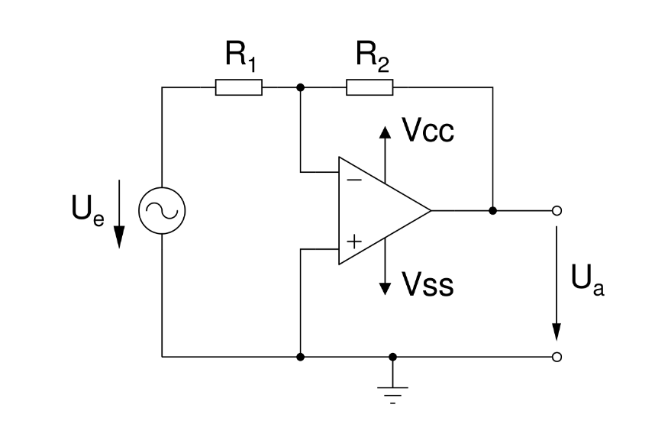
\includegraphics[width=100mm]{i_opv_schaltung.png}
  \caption{Invertierender OPV}
\end{figure}

\subsection*{Durchf\"uhrung}
Die Schaltung wurde gemäß Schaltplan mit dem OPV-IC LM741 aufgebaut. Die Widerstände wurden mit $R_1 = 1k\Omega$ und $R_2 = 47k\Omega$ gewählt um gemäß der Übertragungsfunktion der Schaltung

\begin{figure}[H]
  \centering
  $U_a = -\frac{R_2}{R_1}U_e = -\frac{47k\Omega}{1k\Omega}U_e = -47*U_e$
\end{figure}

\noindent eine 48-fache Verstärkung der Eingangsspannung zu erreichen. Der OPV wurde mit $\pm 15V$ Versorgungsspannung betrieben. Um Ströme und Spannungen in der Schaltung zu messen, wurde ein Eingangsspannung von $0,1V$ angelegt und die Werte in der Folge mit dem Multimeter erhoben. Um das Verhalten des invertierenden OPV im Zeitbereich zu untersuchen, wurde eine Dreieckspannug mit $0,1V_{pp}$ Amplitude und jeweils mit $100Hz$ und $10kHz$ Frequenz angelegt. Hierbei wurden Messungen mit dem Oszilloskop durchgeführt. Um das Frequenzverhalten der Schaltung zu untersuchen wurde jeweils ein Bode-Diagramm für den invertierenden Verstärker mit -47-facher und -4,7-facher ($R_2=4,7k\Omega$) Verstärkung angefertig. Hierfür wurde als Eingangsspannung ein Sinussignal mit $0,1V_{pp}$ gewählt, wobei im Bereich zwischen $10Hz$ und $1MHz$ gemessen wurde.

\subsection*{Ergebnisse \& Diskussion}

% \begin{table}[H]
%   \centering
%   \begin{tabular}{c||c|c|}
%     & $U_e = 0,1V$ & Abweichung\\
%     \hline
%     $U_a$ & $-5,77V$ & $-22,7\%$ \\
%     \hline
%     $U_{R2}$ & $5,69V$ & $-21\%$ \\
%     \hline
%     $U_{R1}$ & $128mV$ & $+28\%$ \\
%     \hline
%     $U_d$ & $35mV$ & $+5147\%$ \\
%     \hline
%     $I_{R2}$ & $123uA$ & $+23\%$ \\
%     \hline
%     $I_{R1}$ & $66uA$ & $-34\%$ \\
%     \hline
%     $I_{+}$ & $-0,02uA$ & $+67\%$ \\
%     \hline
%     $I_{-}$ & $7,38uA$ & - \\
%   \end{tabular}
%   \caption{Messergebnisse bei Gleichspannung mit Abweichungen zur Simulation}
% \end{table}

\begin{table}[H]
  \centering
  \begin{tabular}{c|c}
    & $U_e = 0,1V$ \\
    \hline
    $U_a$ & $-5,77V$ \\
    \hline
    $U_{R2}$ & $5,69V$ \\
    \hline
    $U_{R1}$ & $128mV$ \\
    \hline
    $U_d$ & $35mV$ \\
    \hline
    $I_{R2}$ & $123uA$ \\
    \hline
    $I_{R1}$ & $66uA$ \\
    \hline
    $I_{+}$ & $-0,02uA$ \\
    \hline
    $I_{-}$ & $7,38uA$ \\
  \end{tabular}
  \caption{Messergebnisse bei Gleichspannung}
\end{table}

\noindent Die Verstärkung eines Idealen OPV ist unendlich groß, sie wird jedoch durch die Beschaltung herabgesetzt. Die berechnete Verstärkung der Schaltung beträgt $-47$, bei $U_e = 0,1V$ beträgt die gemessene Verstärkung $-57,7$. Da der Ideale OPV einen unendlich großen Eingangswiderstand hat, kann man auch hier erkennen, dass an den Eingängen nur ein sehr kleiner Strom fließt. Die Differenzspannung, welche beim idealen OPV $0V$ beträgt ist mit $35mV$ bei der realen Beschaltung auch sehr klein.

\begin{figure}[H]
  \centering
  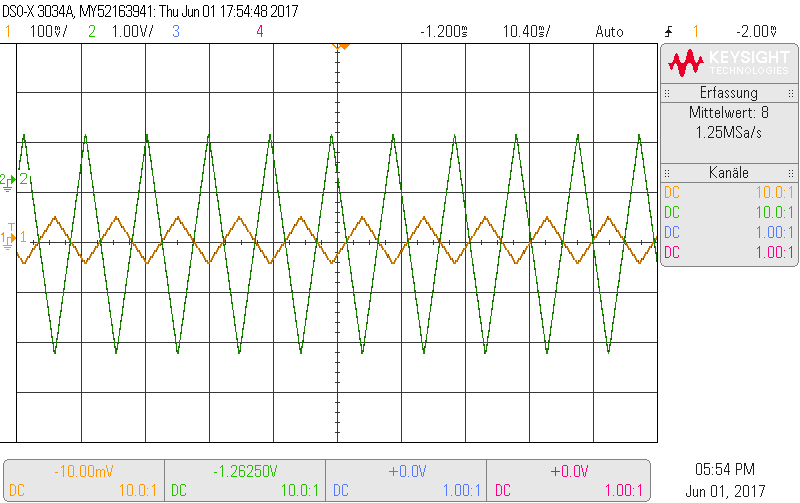
\includegraphics[width=150mm]{scope_5.png}
  \caption{Dreiecksignal mit $100Hz$ (gelb $\hdots\;U_e$, grün $\hdots\;U_a$)}
\end{figure}

\begin{table}[H]
  \centering
  \begin{tabular}{c|c|c}
     & $pp$ & $RMS$ \\
     \hline
    $U_{e}$ & $92mV$ & $28mV$ \\
    \hline
    $U_{a}$ & $4,7V$ & $1,82V$
  \end{tabular}
  \caption{Messungen mit Oszilloskop}
\end{table}

\noindent Das Dreieckssignal wird am Ausgang $-47$-fach (an Spitze-Spitze-Spannung ersichtlich) verstärkt. Am Ausgang ist ein (gegenüber dem Eingang) invertiertes Dreiecksignal erkennbar. Die beiden Signale verlaufen phasengleich.

\begin{figure}[H]
  \centering
  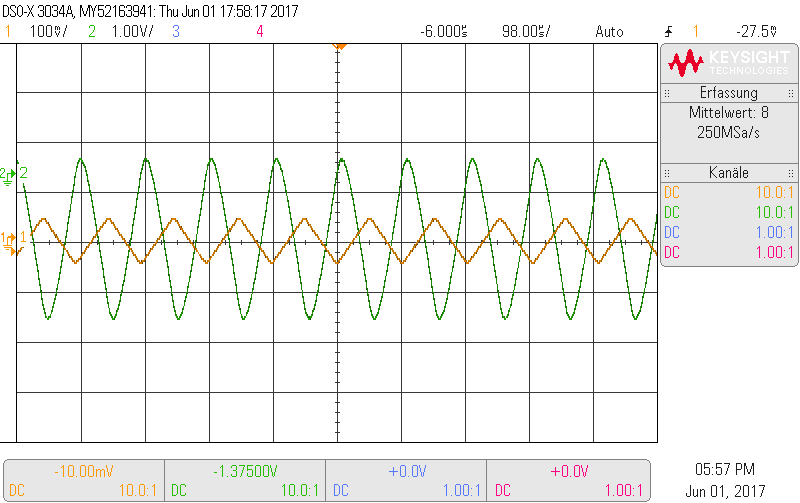
\includegraphics[width=150mm]{scope_7.png}
  \caption{Dreiecksignal mit $10kHz$ (gelb $\hdots\;U_e$, grün $\hdots\;U_a$)}
\end{figure}

\begin{table}[H]
  \centering
  \begin{tabular}{c|c|c}
     & $pp$ & $RMS$ \\
     \hline
    $U_{e}$ & $91mV$ & $27mV$ \\
    \hline
    $U_{a}$ & $3,21V$ & $1,68V$
  \end{tabular}
  \caption{Messungen mit Oszilloskop}
\end{table}

\noindent Bei hoher Frequenz wird die Verstärkung vermindert und das Dreiecksignal wird am Ausgang verschliffen. Dies liegt an der Tiefpasseigenschaft der Verstärkerschaltung, welche nach überschreiten der Grenzfrequenz in Erscheinung tritt.

\begin{figure}[H]
  \centering
  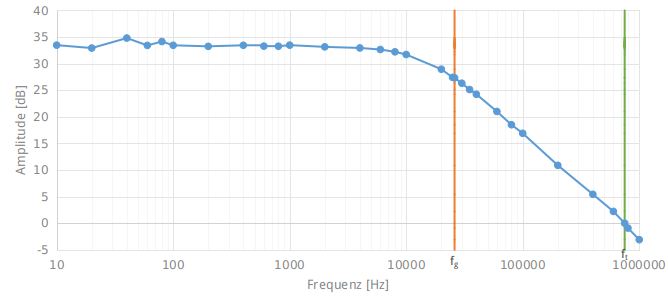
\includegraphics[width=150mm]{bode_47.png}
  \caption{Amplitudengang bei $-47$-facher Verstärkung}
\end{figure}

\noindent Da sich ein OPV intern wie ein Tiefpass verhält, fällt die Verstärkung zwischen Grenzfrequenz ($26kHz$) und Transitfrequenz ($750kHz$) mit einer Filtersteilheit von ca. $-20dB/Dekade$. Bei der Transitfrequenz wird das Signal nicht mehr verstärkt.

\begin{figure}[H]
  \centering
  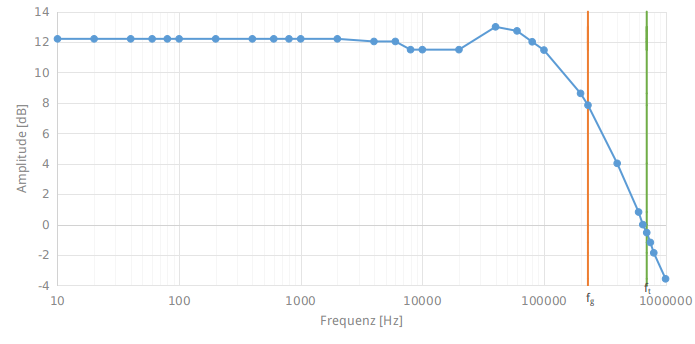
\includegraphics[width=150mm]{bode_4_7.png}
  \caption{Amplitudengang bei $-4,7$-facher Verstärkung}
\end{figure}

\noindent Wenn die Verstärkung der Schaltung verringert wird (auf $\frac{1}{10}$), verschiebt sich die Grenzfrequenz ($230kHz$) in Richtung höherer Frequenzen und die Dämpfung ist erst eine Dekade später zu erkennen. Die Filtersteilheit beträgt jedoch auch hier ca. $-20dB/Dekade$.

\section{Integrierer}

%\subsection*{Notizen}
%gew\"ahlter OPV: LM324 \\
%Integrierer LM324 rechtecksignal $0,1 V_PP$ $5Hz$ scope\_9

\subsection*{Aufgabenstellung}
In der \"Ubung soll eine einfache integrierende Operationsverstärkerschaltung aufgebaut werden. Es sollen die Str\"ome und Spannungen in dieser Schaltung gemessen und dadurch das Verhalten eines Integrierers nachvollzogen werden.

\subsection*{Schaltplan}
\begin{figure}[H]
  \centering
  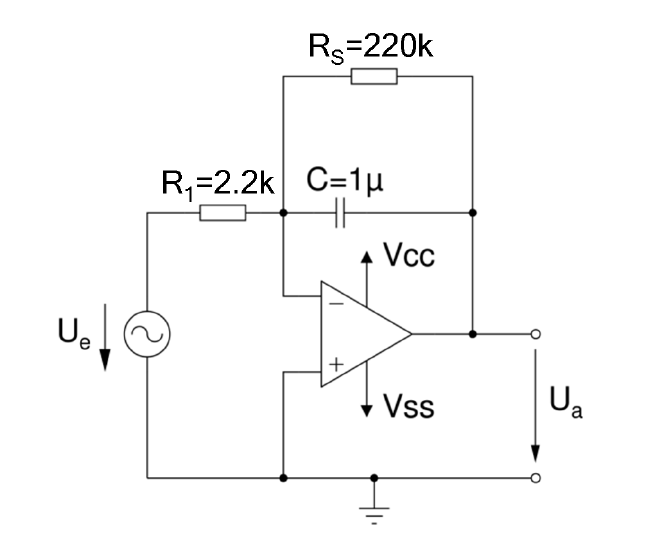
\includegraphics[width=80mm]{integrierer_opv_schaltung.png}
  \caption{Integrierer}
  \label{figure31}
\end{figure}

\subsection*{Durchf\"uhrung}
Die Schaltung wurde gemäß Schaltplan (siehe ~\ref{figure31}) mit dem OPV LM324 aufgebaut. Der OPV wurde mit $\pm 15V$ Versorgungsspannung betrieben. Mittels Funktionsgenerator wurde am Eingang ein periodisches Rechtecksignal mit der Einstellung $0,1 V_{PP}$, Offset $0V$, Duty Circle $50\%$ und Frequenz $5Hz$ angelegt. Die Wirkungsweise wurde untersucht und die Eingangs- und Ausgangsspannung aufgezeichnet.

\subsection*{Ergebnisse \& Diskussion}
\begin{figure}[H]
  \centering
  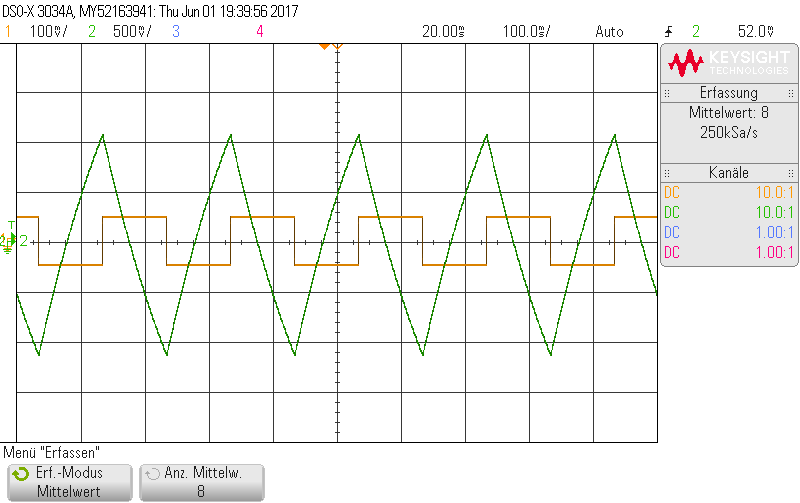
\includegraphics[width=150mm]{integrierer_rechtecksignal_eingang_ausgang.png}
  \caption{Integrierer Rechtecksignal $5Hz$ (gelb \dots $U_e$, gr\"un \dots $U_a$)}
  \label{figure32}
\end{figure}
Ein Integrierer ist ein Verst\"arker, bei dem der Ausgang \"uber einen Kondensator auf den invertierenden Eingang r\"uckgekoppelt wird. Au\ss erdem wird ein hochohmiger Widerstand $R_S$ parallel dazu geschalten, welcher jedoch nur zu Stabilisierung dient. Aufgrund der Kapazit\"at des Kondensators $C$ ergibt sich die \"Ubertragungsfunktion:
\begin{figure}[H]
\centering
$U_a = - \frac{1}{R_1C} \int U_e dt$
\end{figure}
\noindent Am Ausgang erh\"alt man also das invertierte Integral der Eingangsspannung \"uber die Zeit. Wie in der Abbildung~\ref{figure32} zu sehen ist, ergibt sich daher mit einem Rechtecksigal am Eingang ein Dreiecksignal am Ausgang. Verwendung findet die Schaltung bspw. als Teil von PID-Reglern, als aktiver Filter, in der Analogtechnik zum Generieren von S\"agezahnschwingungen oder in Analogrechnern.



\section{Invertierender Schmitt-Trigger}

%\subsection*{Notizen}
%$U_t = 1,719V$\\
%$Ue_{pp} = 5,11V$\\
%$Ua_{pp} = 3,26V$\\
%wenn die amplitude unter die schaltschwelle verringert wird, wird die ausgangsspannung $0V$.

\subsection*{Aufgabenstellung}
In der \"Ubung soll ein invertierender Schmitt-Trigger aufgebaut und dessen Funktionsweise dokumentiert werden.

\subsection*{Schaltplan}
\begin{figure}[H]
  \centering
  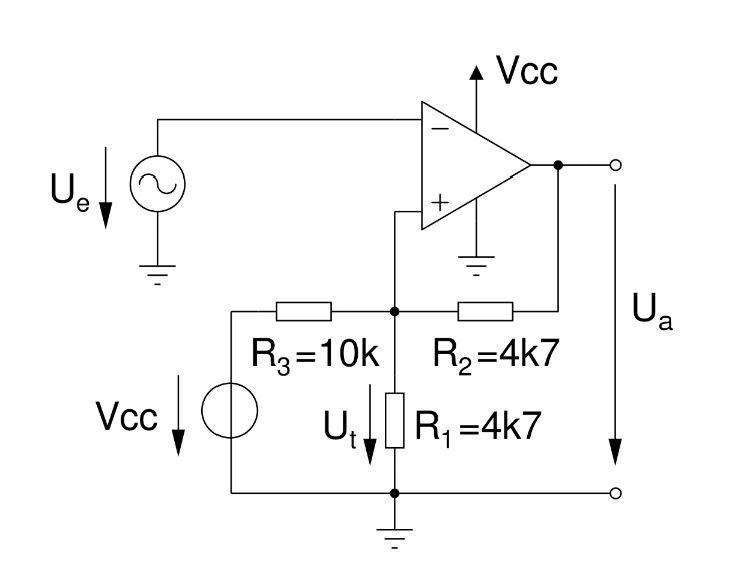
\includegraphics[width=80mm]{i_schmitt_trigger_schaltung.png}
  \caption{Invertierender Schmitt-Trigger}
  \label{figure41}
\end{figure}


\subsection*{Durchf\"uhrung}
Der invertierende Schmitt-Trigger wurde gem\"a\ss \, Schaltplan (siehe ~\ref{figure41}) mit dem OPV LM324 aufgebaut. Am OPV wurde mit $+5V$ am positiven Versorgungsanschluss betrieben, der negative Versorgungsanschluss wurde mit Masse verbunden. Mittels Funktionsgenerator wurde am Eingang ein periodisches Sinussignal mit der Einstellung $5 V_{PP}$, Offset $2,5V$ und Frequenz $50Hz$ angelegt. Die Spannungen $U_a$, $U_e$ und $U_t$ wurden gemessen und protokolliert (siehe Tabelle ~\ref{figure42}). Weiters wurden Eingangs- und Ausgangssignal mit dem Oszilloskop im Zeit- und Bildbereich aufgezeichnet (siehe Abbildung~\ref{figure43} und ~\ref{figure44}).

\subsection*{Ergebnisse \& Diskussion}
\begin{table}[H]
  \centering
  \begin{tabular}{c|c}
    $U_e (PP)$ & $5,11V$ \\
    \hline
    $U_a (PP)$ & $3,26V$ \\
    \hline
    $U_t (PP)$ & $1,72V$
  \end{tabular}
  \caption{Messung Spannungen Invertierender Schmitt-Trigger}
  \label{figure42}
\end{table}
Allgemein schaltet ein Schmitt-Trigger am Ausgang zwischen der positiven bzw. negativen Versorungsspannung um. Die Schaltschwellen, wo das Ausgangssignal kippt sind im Allgemeinen symmetrisch zur Nullline. Um nun die Schaltschwellen auf ein anderes Spannungsniveau zu \"andern, welches nicht symmetrisch zur Nulllinie ist, wird der OPV unipolar und mit einer Referenzspannung betrieben. Dh. die negative Versorgungsspannung mit Masse verbunden. Die positive bzw. negative Versorungsspannung wird hier nicht erreicht, da es sich hier um eine Rail-To-Rail OPV Schaltung handelt.

\begin{figure}[H]
  \centering
  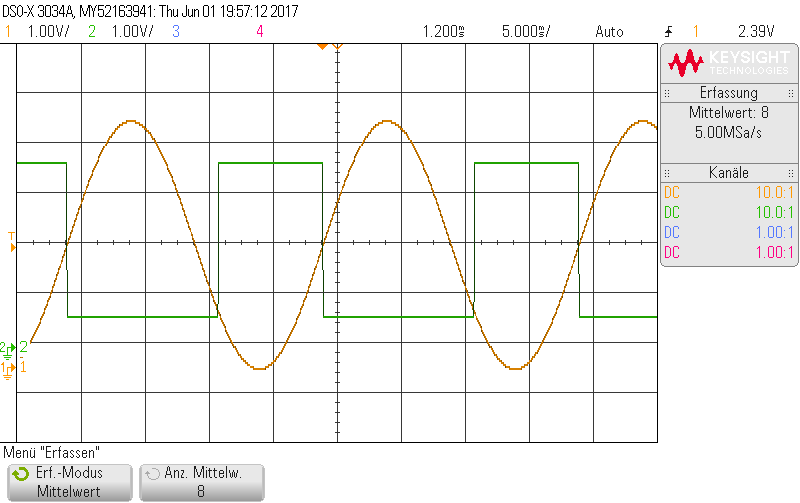
\includegraphics[width=150mm]{i_schmitt_trigger_sinus.png}
  \caption{Invertierender Schmitt-Trigger mit $50Hz$ Sinussignal (gelb \dots $U_e$, gr\"un \dots $U_a$)}
  \label{figure43}
\end{figure}
\noindent Der Schmitt-Trigger arbeitet als Komparator mit Hysterese. Das bedeutet, dass die beiden Eing\"ange (invertierend und nichtinvertierend) verglichen werden und der Ausgang schaltet entsprechend auf $U_{low}$ bzw. auf $U_{high}$. Wie in Abbildung ~\ref{figure43} zu erkennen ist, h\"angen $U_e$ und $U_a$ so zusammen, dass bei den Schwellwerten ($\approx 1V$ und $~\approx 2,5V$) der Ausgang entweder auf $\approx 0,6V$ bzw. auf $\approx 3,8V$ kippt. Die Spannung $U_t$ ist direkt proportional zu $U_a$. Diese Kippstufe kommt daher, dass ein Teil der Ausgangsspannung auf den positiven Eingang des OPV zur\"uckgef\"uhrt wird (Mitkopplung). Allgemein ben\"otigt man die Hysterese, da sonst im Bereich der Schaltschwelle die Ausgangsspannung mehrfach kippen k\"onnte.\\
Bei der Ausgangsspannung $U_a$ ist mit $0,6V$ bzw. $3,8V$ ein Unterschied zu den berechneten Werten aus der Simulation zu erkennen ($0,029V$ bzw. $4,39$). Dies kommt daher, dass bei der Berechnung ideale Bauelementen angenommen werden. Wird die Amplitude des Eingangssignals verringert, so kann man sehen, dass der Schmitt Trigger am Ausgang nicht mehr schaltet.


\begin{figure}[H]
  \centering
  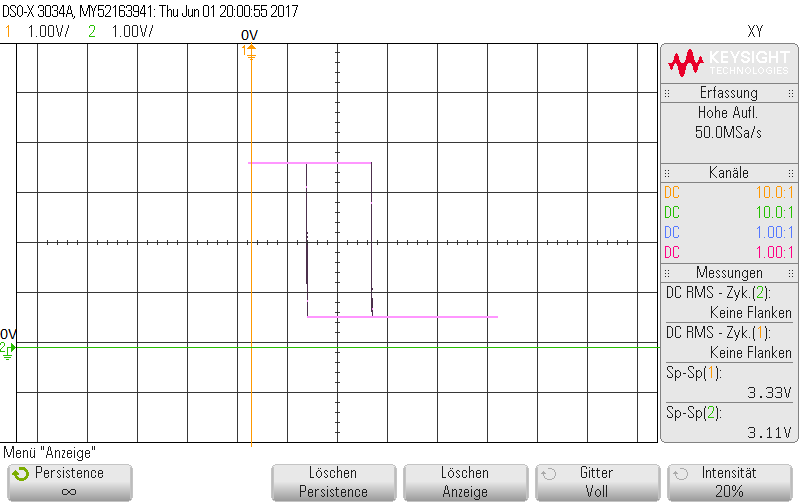
\includegraphics[width=150mm]{i_schmitt_trigger_hysterese_kennlinie.png}
  \caption{Invertierender Schmitt-Trigger mit Sinussignal (Bildbereich); x-Achse: $U_e$; y-Achse: $U_a$}
  \label{figure44}
\end{figure}
\noindent Die Abbildung ~\ref{figure44} zeigt die Hysterese-Kennlinie des invertierenden Schmitt-Triggers. Auf der x-Achse ist die Eingangsspannung und auf der y-Achse die Ausgangsspannung eingtragen. Der Verlauf sieht so aus, dass die Linie links oben startet. Die Eingangsspannung wird erh\"oht, ohne dass sich die Ausgangsspannung \"andert. Wird der obere Schwellwert des Schmitt-Triggers erreicht (rechts oben), so schaltet der Ausgang auf $U_{low}$. Danach steigt die Eingangsspannung weiter, ohne \"Anderung am Ausgang. Da es sich um ein periodisches Sinussignal handelt, sinkt dann die Eingangsspannung wiederum bis auf den unteren Schwellwert und der Ausgang schaltet wider auf $U_{high}$. \\
% TODO: Wird die Art des Eingangssignals ge\"andert, so \"andert sich auch das Bild der Hysterese-Kennline, jedoch ist immer ein geschlossener Kreis zu erkennen. Der Unterschied liegt immer.\\
\noindent Verwendet wird diese Schaltung bspw. zum Erzeugen von bin\"aren Signalen oder um eindeutige Schaltzustände aus einem analogen Eingangssignalverlauf zu gewinnen.

%\begin{figure}[H]
%  \centering
%  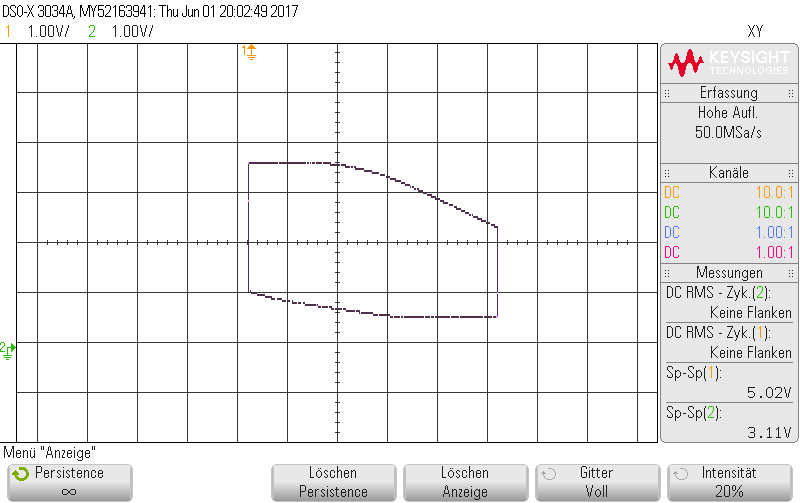
\includegraphics[width=150mm]{scope_15.png}
%  \caption{Invertierender Schmitt-Trigger mit Dreiecksignal (Bildbereich)}
%\end{figure}


\section{Anhang - Messwerte}

\begin{figure}[H]
  \centering
  \begin{minipage}[b]{0.4\textwidth}
    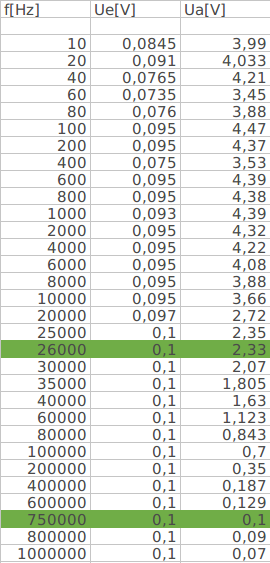
\includegraphics[width=\textwidth]{daten_47.png}
    \caption{Messdaten invertierender OPV (-47 Verstärkung)}
  \end{minipage}
  \hfill
  \begin{minipage}[b]{0.4\textwidth}
    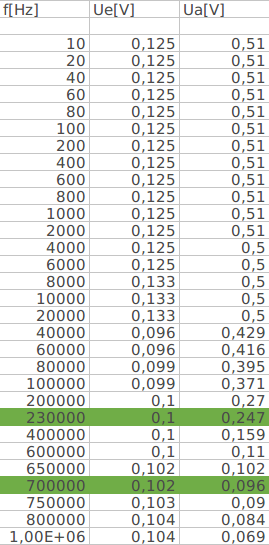
\includegraphics[width=\textwidth]{daten_4_7.png}
    \caption{Messdaten invertierender OPV (-4,7 Verstärkung)}
  \end{minipage}
\end{figure}

\end{document}
